\section{几何}

\subsection{三角函数}
\subsubsection{$\protect\sin x\ \text{和}\ \cos x$}
\begin{proof}
    
\begin{figure}[H]
    \centering
    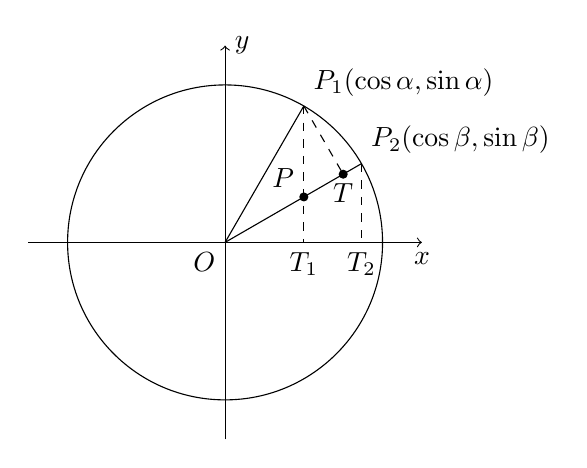
\begin{tikzpicture}
        \draw[->](-2.5, 0)--(2.5, 0)node[below]{$x$};
        \draw[->](0, -2.5)--(0, 2.5)node[right]{$y$};
        \node[below left]at(0, 0){$O$};
        \draw(0, 0) circle(2);
        \draw(0, 0) --(60:2) node[above right]{$P_1(\cos\alpha, \sin\alpha)$};
        \draw[dashed](60:2)--(60:2|-0,0) node[below]{$T_1$};
        \draw(0, 0) --(30:2) node[above right]{$P_2(\cos\beta, \sin\beta)$};
        \draw[dashed](30:2)--(30:2|-0,0) node[below]{$T_2$};
        \node[above left] at(1,{sqrt(1/3)}){$P$};
        \draw[dashed](60:2)--(30:{sqrt(3)}) node[below]{$T$};
        \filldraw[black](1,{sqrt(1/3)})circle(0.05);
         \filldraw[black](30:{sqrt(3)})circle(0.05);
    \end{tikzpicture}
    \caption{\(\dis
    \left\{\begin{matrix} 
    \sin(\alpha - \beta) = \sin\alpha\cos\beta -\cos\alpha\sin\beta\\
  \cos(\alpha - \beta)=\cos\alpha\cos\beta + \sin\alpha\sin\beta
\end{matrix}\right.
    \)的几何证明}
    \label{fig:sin-cos-substract-proof}
\end{figure}
已知\(\odot O\)的半径\(R=1\)，\(\angle xOP_1=\alpha,\ \angle xOP_2=\beta\)，\(
P_1T\perp OP_2,\ P_1T_1\perp Ox,\ P_2T_2\perp Ox
\)

易得，\(\dis \angle POT_1 = \angle PP_1P_2,\ PT_1 = \cos\alpha\tan\beta, OP = \frac{OT_1}{\cos\beta} = \frac{\cos\alpha}{\sin\beta},\ PT =P_1P\sin\beta = (\sin\alpha - \cos\alpha\tan\beta)\sin\beta,\ P_1T=P_1P\cos\beta=(\sin\alpha - \cos\alpha\tan\beta)\cos\beta \)
则：
\begin{align*}
    \sin(\alpha - \beta) &= P_1T\\
    = \sin\alpha\cos\beta &-\cos\alpha\sin\beta
\end{align*}

\begin{align*}
    \cos(\alpha - \beta)&=OP + PT\\
    =\frac{\cos\alpha}{\cos\beta} &+ (\sin\alpha -\cos\alpha\tan\beta)\sin\beta
    \\=\frac{(\sin^2\beta + \cos^2\beta)\cos\alpha}{\cos\beta}&+\frac{\sin\alpha\sin\beta\cos\beta - \sin^2\beta\cos\alpha}{\cos\beta}
     \\=\cos\alpha\cos\beta &+ \sin\alpha\sin\beta
\end{align*}




\end{proof}

\subsubsection{$\protect\tan x$}

\begin{figure}[H]
    \centering
    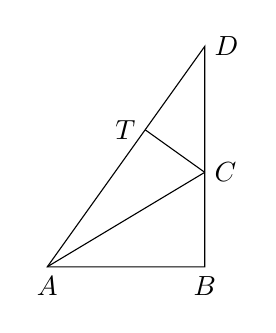
\begin{tikzpicture}[scale=2]
        \draw(0, 0)node[below]{$A$} --(1, 0)node[below]{$B$}
        --(1, 0.6)node[right]{$C$}
        --(1, 1.4)node[right]{$D$}--cycle;
        \draw(0, 0)--(1, 0.6);
        \draw(23/37, 161/185)node[left]{$T$} -- (1, 0.6);
    \end{tikzpicture}
    \caption{$\dis\tan(\alpha-\beta) = \frac{\tan\alpha-\tan\beta}{1+\tan\alpha\tan\beta}$的几何证明}
    \label{fig:enter-la}
\end{figure}

已知\(\angle BAD = \alpha,\ \angle CAB=\beta, AB=1, CT\perp AD\)，
\begin{proof}
可得\[
DB = \tan\alpha,CB=\tan\beta,CD=\tan\alpha - \tan\beta
\]
\[
\tan(\alpha - \beta) = \tan\angle CAD=\frac{CT}{AT}
\]
可以得出\(\angle BAD = \angle DCT, TD = \tan(\alpha - \beta)\cos\alpha, CT = \tan(\alpha - \beta)\sin\alpha\)
\end{proof}

\subsection{外心}
\begin{figure}[H]
    \centering
    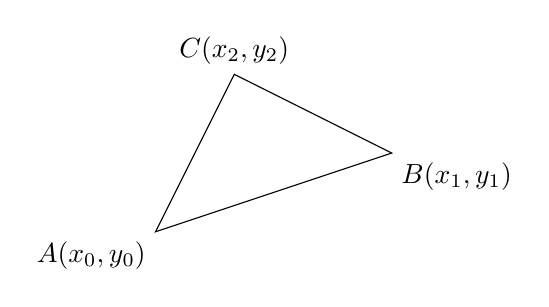
\begin{tikzpicture}
    \draw(-1, -1) node[below left]{$A(x_0, y_0)$}--(2,0)node[below right]{$B(x_1, y_1)$}--(0, 1)node[above]{$C(x_2, y_2)$}--cycle;
\end{tikzpicture}
    \caption{Caption}
    \label{fig:enter-label}
\end{figure}
设外心的坐标为$T(a, b)$, 则
\begin{align*}
    (a - \frac{x_1+x_0}{2}, b-\frac{y_1+y_0}{2})&\cdot
(x_1-x_0, y_1-y_0) = 0\\
(a - \frac{x_2-x_0}{2}, b-\frac{y_2-y_0}{2})&\cdot
(x_2-x_0, y_2-y_0) = 0\\
\end{align*}
即
\begin{align*}
    a(x_1-x_0)+b(y_1-y_0) = \frac{x_1^2-x_0^2}{2}+\frac{y_1^2-y_0^2}{2}\\
    a(x_2-x_0)+b(y_2-y_0) = \frac{x_2^2-x_0^2}{2}+\frac{y_2^2-y_0^2}{2}\\
\end{align*}
利用上面两个方程，解出$a, b$即可。即
\begin{align*}
    a(x_1-x_0)+b(y_1-y_0) = \frac{x_1^2-x_0^2}{2}+\frac{y_1^2-y_0^2}{2}\\
    a(x_2-x_0)+b(y_2-y_0) = \frac{x_2^2-x_0^2}{2}+\frac{y_2^2-y_0^2}{2}\\
\end{align*}